\section{CSS}

L’obbiettivo principale che ogni programmatore Web si pone nella fase di progettazione della struttura del proprio sito è quello di farne apparire i contenuti nel modo più chiaro ma allo stesso tempo accattivante possibile. Nel realizzare la struttura del sito "Le vecchie credenze" abbiamo quindi puntato ad ottenere un design assolutamente pulito, privo di ogni possibilità di confusione, che permette l' immediata comprensione dei contenuti anche da parte di un utente casuale. 

\subsection{La struttura}
Le principali sezioni che compongono il nostro sito sono  navigation e content.

\paragraph{Navigation}

Questa sezione contiene il banner ufficiale del sito seguito dal menu a lista attraverso il quale è possibile accedere a tutte le pagine attraverso gli appositi link. Questa sezione contiene anche il footer in cui sono presenti le indicazioni necessarie a raggiungere il ristorante e il link alla sezione “Credits”, che contiene alcune informazioni sui progettatori del sito, “Admin” che permette l’accesso alla pagina di amministrazione e i link ai validatori W3C.


\begin{figure}[H]
		\centering 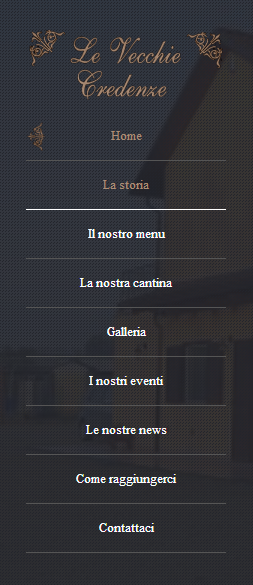
\includegraphics[width=0.4\textwidth]{images/navigation.png}
		\caption{Sezione navigation}
\end{figure}

\begin{figure}[H]
		\centering 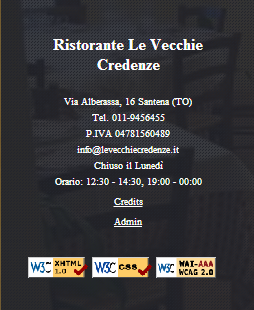
\includegraphics[width=0.4\textwidth]{images/footer.png}
		\caption{Sezione occupata dal footer}
\end{figure}

\paragraph{Content}

Questa sezione invece contiene i contenuti veri e propri presentati nelle pagine del sito, introdotti sempre da un titolo.

\begin{figure}[H]
		\centering 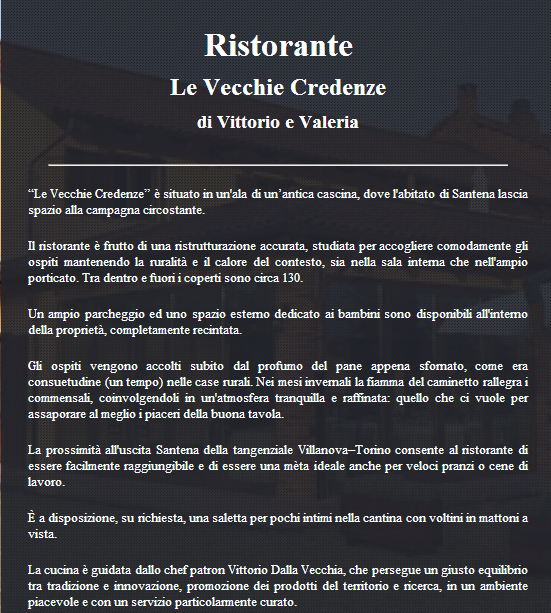
\includegraphics[width=0.4\textwidth]{images/content.png}
		\caption{Sezione dedicata ai contenuti}
\end{figure}

\subsection{L’utilizzo delle mediaquery}

Per affrontare il problema della intercompatibilità tra le varie piattaforme abbiamo utilizzato le mediaquery che linkano ai diversi CSS adattati alle dimensioni dello screen della piattaforma stessa da cui si sta effettuando l’accesso al sito.

\subsection{I colori}

\paragraph{Background}

Per la visualizzazione della pagina a schermo intero abbiamo utilizzato una slide show di immagini mentre per le versioni per tablet e smartphone questa è stata rimpiazzata da uno sfondo monocromatico per rendere più leggera e chiara la visualizzazione dei contenuti.

\paragraph{Link}

Per i link del campo content si è deciso di scegliere un colore oro per i link visitati mentre per i selected abbiamo mantenuto il colore “standard” del sito che riprende stilisticamente il banner presente in navigation. Per quanto riguarda i link del menu presente in navigation abbiamo deciso, pur essendo consapevoli del fatto che al fine di rendere un sito accessibile sarebbe opportuno cambiare il colore dei link visitati anche al menu di navigazione, di mantenere un colore classico (bianco) per evitare confusione o effetti spiacevoli alla vista poiché il principale obbiettivo è di creare una vetrina per un ristorante quindi deve essere quanto più piacevole alla vista possibile. 

\begin{figure}[H]
		\centering 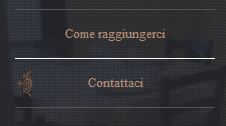
\includegraphics[width=0.4\textwidth]{images/link-navigation.png}
		\caption{Link della sezione navigation}
\end{figure}

\begin{figure}[H]
		\centering 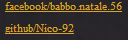
\includegraphics[width=0.4\textwidth]{images/link-content.png}
		\caption{Effetto per i link visistati presenti nel content}
\end{figure}

\subsection{CSS3}

Le proprietà del nuovo standard che abbiamo utilizzato nel nostro progetto sono:

\paragraph{Background-size}

Utilizzato per regolare la grandezza delle immagini di background  della slide show e del banner.

\paragraph{Border- radius}

Utilizzato per arrotondare i margini nella sezione social e nelle immagini della sezione credits.

\paragraph{box-shadow}
Questa proprietà è stata implementata nei form della parte di amministrazione, qualora l' amministratore cerchi di eseguire l' input di un form avendo lasciato dei campi obbligatori vuoti, tali campi verranno evidenziati con un' aura rossa abbastanza evidente in modo da essere anche accessibile.
\begin{figure}[H]
		\centering 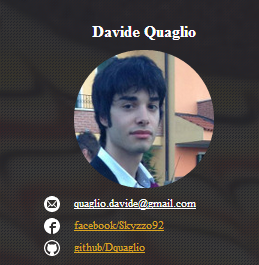
\includegraphics[width=0.5\textwidth]{images/radius.png}
		\caption{Utilizzo della proprietà radius nella pagina Contattaci}
\end{figure}

\paragraph{Si ricorda che}

Abbiamo inoltre utilizzato la proprietà webkit che non è parte attualmente degli standard css ma gli ultimi aggiornamenti del validatore w3c hanno declassato tali errori a warning, e si sta valutando di aggiungere webkit allo standard.

\begin{figure}[H]
		\centering 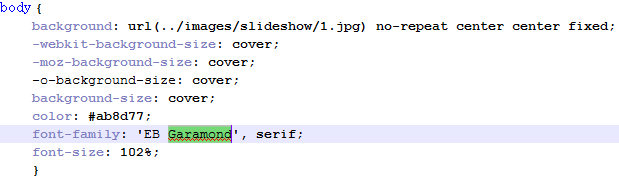
\includegraphics[width=0.4\textwidth]{images/webkit.png}
		\caption{Utilizzo della proprietà webkit nel Body}
\end{figure}

\subsection{Note importanti}

\paragraph{Font}

Abbiamo scelto di utilizzare un font più elaborato (Garamond) poiché il sito è creato come vetrina per un ristorante e quindi abbiamo privilegiato l’immagine e l’impatto estetico a scapito dei tempi di caricamento delle pagine stesse anche se la differenza in velocità è pressoché impercettibile.
